\chapter{Background and selection criteria}
\label{chp:LitSurvey}
In this chapter, a state-of-the-art study will be presented that would assist in the design of the lensless imager that can be used onboard the Delfi-PQ Satellite. This chapter also provides background information that will be useful in understanding the concepts covered in the later chapters. 
\section{Camera Computational Pipeline}
In order to design a lensless imaging system, we must first look at the computational imaging pipeline of existing cameras. Since the lensless camera basically uses computation to reconstruct images, it is important to understand the computational pipeline of existing camera systems and make necessary modification in the design of the existing pipeline to suit the system. The computational imaging pipeline of existing camera systems is shown figure \ref{fig:CompPipeline}\cite{CompPipeline}.
\begin{figure}[htb]
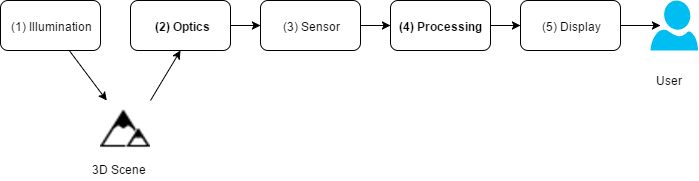
\includegraphics[width=\textwidth]{pics/CompPipeline}
\caption{Computational Pipeline of Existing cameras}
\label{fig:CompPipeline}
\end{figure}
As shown in figure \ref{fig:CompPipeline}, there are five main components that can be controlled computationally in existing systems. Illumination of the scene can be controlled to produce an enhanced picture. Optics could be controlled to limit the amount of light entering the sensor and thereby controlling the image produced by the sensor. The sensor can also computationally modify the date it receives to de-noise, adjust the blackness/white in an image. Post-processing can also be done on the image produced by the sensor to improve the image produced by the sensor. Finally, a display can also be modified computationally to produce certain effects on the user. And of course, the user can control any of these components to produce the effect he desires. But in the case of the lensless imaging system, we would be modifying the optics and the processing components of the pipeline to reduce the size of the camera. The components to be modified are darkened in figure \ref{fig:CompPipeline}. 

\section{Satellite Imaging Architectures}
Since the camera is going to be capturing pictures of the earth, it would be required to study the existing imaging architectures currently being used in satellites and how the design of the lensless camera would fit into the existing imaging architectures. We will first look into the terminology commonly used in space instrumentation. As the imager is carried along the orbit of the earth, it images a strip on the surface of the earth. The width of the strip is called the `swath'. The direction along which the satellite moves or images is called the `along-track' direction and the direction perpendicular to it is called the cross-track direction\cite{ImagingGeo}. Figure \ref{fig:ImagingGeo} describes this terminology and some other terms as well.  
\begin{figure}[ht]
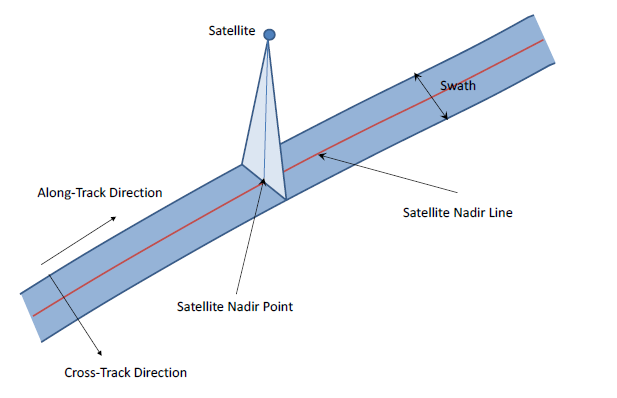
\includegraphics[width=\textwidth]{pics/imaginggeo}
\caption{Various Imaging Terms\cite{ImagingGeo}}
\label{fig:ImagingGeo}
\end{figure}
Three major types of scanning architectures are employed in space instruments, namely:
\begin{itemize}
\item Whiskbroom Line Scanner: In this type of scanning architecture, a detector element detects it's instantaneous field of view which is projected onto a pixel element. In this scanning type, the surface of the earth is scanned in lines. A scanning mirror would project a very small area of the earth onto the single pixel element. The scanning mirror would then rotate to project the next element of the line onto the next pixel. Depending on the motion of the satellite, the next line of the detector is scanned and projected on to the next line on the surface of the earth. An advantage of this type of detector is that it would be possible to obtain a very large field of view. However, it also comes with a disadvantage that a very high sampling frequency is required to get decent resolutions. Typically, an earth observation satellite would move at 6.5 km per second. In order to get a resolution of 100 meters per pixel, it would be required to sample at least 65 lines per second. For a swath of 1000 pixels, it would be required to sample at 65000 elements per second. Apart from this, there is very limited time for each detector element which would result in low spatial resolution\cite{SpInst}. Another main disadvantage is that mechanical components would be required to project different parts of the surface of the earth on to the detector element. This type of scanner is also called as the along-track scanner. Mathematically, the measurement of the detector element $(X, Y)$ can be described using 
$$
(X, Y) = f(t_x, t_y)
$$
where $t_x$ and $t_y$ is the time at which the image is captured in the corresponding location
%\begin{figure}[ht]
%\begin{subfigure}
%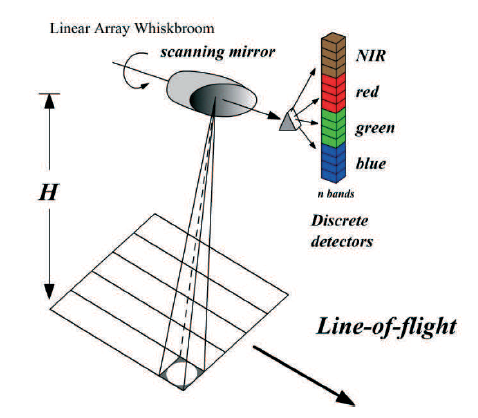
\includegraphics[width=0.5\textwidth]{pics/WhiskBroom}
%\caption{Whiskbroom Scanning Architecture}
%\label{fig:WhiskBroom}
%\end{subfigure}
%\begin{subfigure}
%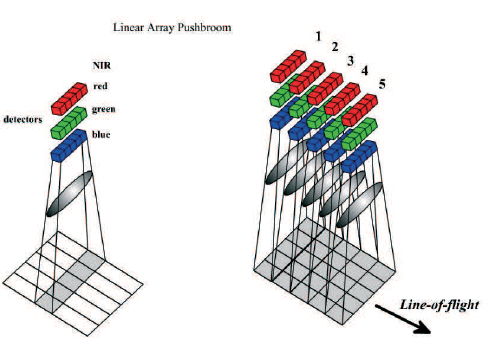
\includegraphics[width=0.5\textwidth]{pics/PushBroom}
%\caption{Pushbroom Scanning Architecture}
%\label{fig:PushBroom}
%\end{subfigure}
%\end{figure}
\begin{figure}[ht]
\centering
\begin{subfigure}{0.80\textwidth}
  \centering
  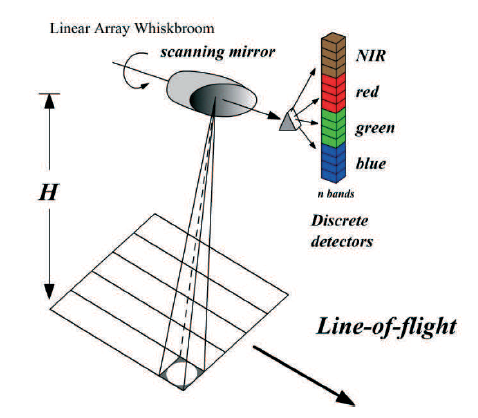
\includegraphics[width=0.75\linewidth]{pics/WhiskBroom}
  \caption{WhiskBroom Scanning}
  \label{fig:Whiskbroom}
\end{subfigure}
\begin{subfigure}{0.80\textwidth}
  \centering
  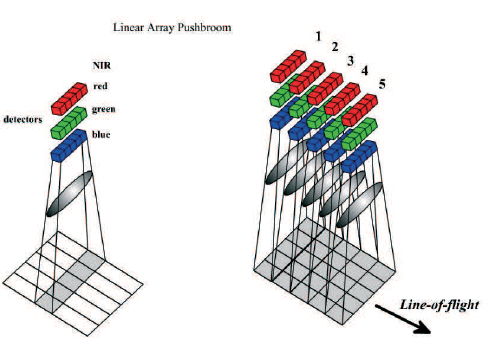
\includegraphics[width=0.75\linewidth]{pics/PushBroom}
  \caption{Pushbroom Scanning}
  \label{fig:Pushbroom}
\end{subfigure}
\caption{Push Broom and Whisk Broom Scanning\cite{SpInst}}
\label{fig:test}
\end{figure}

\item Pushbroom Line Scanner: In this type of architecture, the orbital motion of the sensor is used to image the swath instead of using a mirror as in the case of whiskbroom scanner. The field of view in the cross-track direction is imaged by the corresponding line detector array. Successive lines are imaged and sampled by the multiplexer as the sensor moves across the surface. The time between sampling two successive lines can be the time it takes for the satellite to move that distance. The most commonly used detector for a push broom scanner is Charge Coupled Devices(CCD). One of the main advantages of this type of scanner is that it requires no moving parts. Due to this, it is possible to obtain very high scanning rates( $\leq 1 \mu$ second). This also leads to lower noise in the received signal\cite{SpInst}. The disadvantage is that a large number of detectors are required to image a large piece of an area of the earth. In addition to this, it requires an optical arrangement that could obtain a wide field of view. Mathematically, the measurement of the detector element $(X, Y)$ can be described using 
$$
(X, Y) = f(x), f(t_y)
$$
where $f(x)$ represents the sensor output and $f(t_y)$ represents the time at which the subsequent rows are imaged.  
\item Staring Array: Staring arrays use 2-D CCD/CMOS detectors to capture an entire area on the surface of the earth. These are also called as framing cameras. This provides speed-up and step-and-stare mechanism is employed wherein observations are made intermittently after a certain number of steps in the cross-track direction. The advantage is that moderate field of view optics is only required in this case\cite{SpInst}. Mathematically, the measurement of the detector element $(X, Y)$ can be described using 
$$
(X, Y) = f(x), f(y)
$$
where $f(x)$ and $f(y)$ represents the sensor output.
\end{itemize}

\section{Spatial Resolution and Field of View}
Two important factors that come into account when developing cameras for space applications are the spatial resolution and field of view. These factors determine the performance of the camera and it is important to know how these cameras will perform when designed.


\subsection{Spatial Resolution}
Spatial resolution in remote sensing refers to the smallest area represented by the pixel element of the detector. The impact of different spatial resolutions on imaging a house object is shown in Figure \ref{fig:spatial_resolution}. For example, if a house on earth measures $30 \ m \times 30 \ m$, a camera with a spatial resolution of $30 \  m$ cannot image the house completely and the pixel is going to be the average color of that particular area which is 30m. If the spatial resolution is reduced to $5 \ m$, then we can differentiate between different components of the house. An even smaller spatial resolution of $1 \ m$ will enable us to see the finer details of the house components. 

\begin{figure}[htb]
\centering
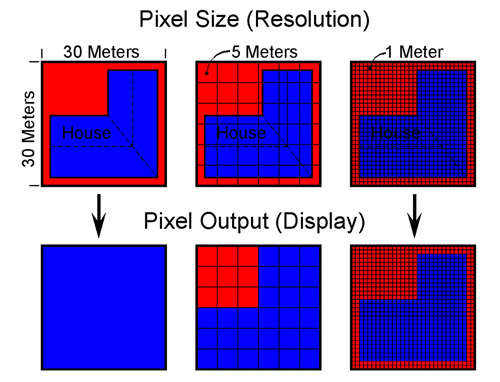
\includegraphics[width=0.75\textwidth]{pics/spatial-resolution}
\caption{Picture Quality variation according to different spatial resolutions\cite{SpatialResol}}
\label{fig:spatial_resolution}
\end{figure}

In remote sensing, a system with high spatial resolution is one which has a resolution of $0.41-4 \  m$ per pixel, a system with low spatial resolution has a resolution ranging from $30-1000 \ m$ per pixel\cite{SpatialResol}. The spatial resolution of a system can be determined by the equation \ref{eq:spat_res}. 

\begin{equation}
\label{eq:spat_res}
d_s = \frac{d_p}{d_t} * d_h
\end{equation}
where $d_s$ indicates the spatial resolution, $d_p$ indicates the individual pixel size of detector element, $d_h$ indicates the height of the instrument from earth and $d_t$ indicates the thickness of the camera or the distance of the lens/mask from the sensor.

The equation \ref{eq:spat_res} is obtained by using the simple triangular rules and the relation can be obtained by using Figure \ref{fig:spatial_resolution_calc}.
\begin{figure}[htb]
\centering
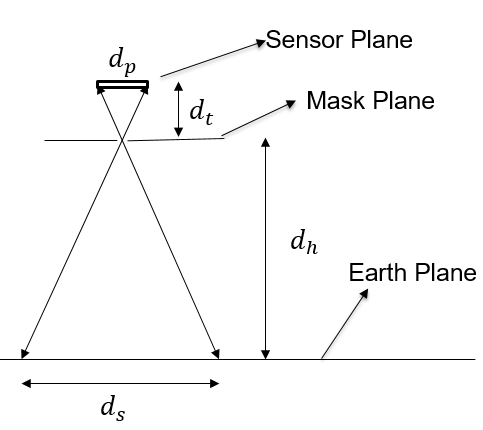
\includegraphics[width=0.75\textwidth]{pics/spatialRes}
\caption{Spatial Resolution Calculation}
\label{fig:spatial_resolution_calc}
\end{figure}

\subsection{Field of View}
The field of view is the amount of area of the surface of the earth that can be imaged by the sensor. In a lens-based system, the field of view is determined by the chief ray angle of the lens in use. In a lensless system, the field of view is determined by the acceptance angle of the CMOS/CCD sensor in use. The field of view can be determined by the equation \ref{eq:fov_calc}.
\begin{equation}
\label{eq:fov_calc}
d_{fov} = 2*d_h*tan(\theta_{cra})
\end{equation}
where $d_{fov}$ is the area that can be imaged by the sensor, $d_h$ determined the height of the instrument from the surface of the earth and $\theta_{cra}$ is the acceptance cone or the acceptance angle of the sensor elements. This equation can be determined by using simple triangular laws and this is shown in Figure \ref{fig:fov_calc}.
\begin{figure}[htb]
\centering
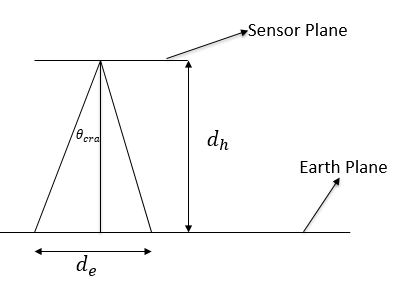
\includegraphics[width=0.75\textwidth]{pics/fov}
\caption{Field of View Calculation}
\label{fig:fov_calc}
\end{figure}
Sensors used by the Landsat program(program by NASA for earth observation satellites) have a field of view of $185 \ km \times 185 \ km$ at a height of 705 kilometers from the surface of the earth\cite{landsat}.

\section{Trade-off Analysis}
\label{sec:tradeOff}
\subsection{Camera Sensor}
The camera sensor is the core of the Delfi-PQ Imager. The performance of a camera is mainly limited by the image sensor that it uses. The camera sensor can be of two types namely, CCD(charge coupled device) or CMOS(Complementary Metal Oxide Semiconductor). Both the types of sensors have their own advantages and disadvantages. To understand the challenges that each type of sensor poses, we must understand how the sensors are designed. The image sensor typically contains a two-dimensional array of sensors that convert the incoming light into electrical signals. To obtain imaging in the visible light domain, a color filter is added over the top of the array of pixels, that filter and allow only the red, green and blue components. The analog voltage is then converted to digital data using and then the process of demosaicking is used to convert the image intensity map to the actual object image \cite{cmos}. The image sensor has a micro-lens array in order to increase the amount of light incident on the surface of the sensor. In a lensless system, the field of view of the camera is also determined by the acceptance angle of the micro-lens array(See Figure \ref{fig:cmos_micro}).

\begin{figure}[ht]
\centering
\begin{subfigure}{\textwidth}
  \centering
  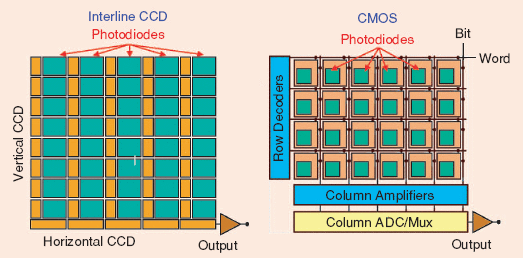
\includegraphics[width=\linewidth]{pics/cmos/cmosccd}
  \caption{Readout architectures of CMOS and CCD}
  \label{fig:cmos_ccd}
\end{subfigure}
\begin{subfigure}{0.75\textwidth}
  \centering
  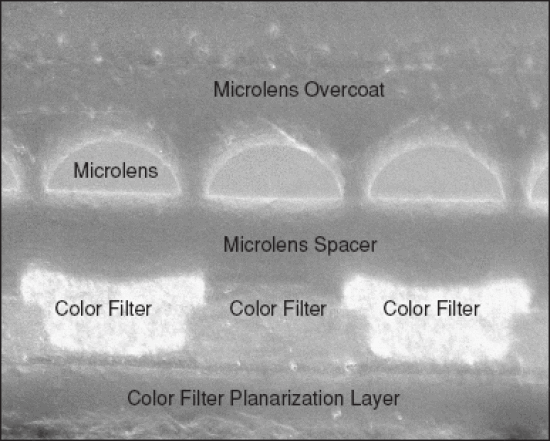
\includegraphics[width=.75\linewidth]{pics/cmos/cmosmicro}
  \caption{Micro lens array and other components in a image sensor}
  \label{fig:cmos_micro}
\end{subfigure}
\caption{Image Sensor Architectures\cite{cmos}}
\label{fig:cmos_1}
\end{figure}

The difference in CMOS and CCD sensors mainly lie in the readout architectures. In CCDs, the electrical charge is shifted out through the horizontal and vertical detector elements and are converted to a voltage through an amplifier. In CMOS sensor image architecture, the charge is read out one row at a time similar to RAM using row-column select switches\cite{cmos}. The architecture of the CCD makes it possible to design sensors with very small pixel-sizes and also leads to lesser readout noise. The CMOS architecture enables extremely fast readout but introduces additional fixed pattern noise and temporal noise due to the introduction of circuitry in each pixel. Manufactures produce both CMOS and CCD types of sensors and we can choose an architecture depending on the type of application. 

These CMOS/CCD sensors can be categorized under the starring array type of imaging architectures that we mentioned previously. The following factors have been chosen to  make a trade-off between the different image sensors available on the market:
\begin{enumerate}
\item Resolution: When rating a camera, the first thing that comes to the mind is the resolution of the camera. The resolution of a camera is directly dependent on the number of pixels in the image sensor of the camera. 
\item Power Consumption: In the design of the imager, the most important factor is the power consumption of the entire imager. The majority of the power consumption by the imager is dependent on the power consumption of the image sensor. 
\item Availability: Even though there is an innumerable number of image sensors in the world, availability of image sensors is quite low when it comes to small-scale production. Many image sensor manufacturers require large-scale orders.
\item Quantum Efficiency(QE): Quantum Efficiency is the measure of the efficiency of the camera sensor to convert incoming photons into electrons. The ratio of electrons generated during the digitization process to photons is called quantum efficiency. This factor is extremely important, however, most manufacturers do not provide this information. This factor is ignored since a majority of the cameras studied do not specify this information.
\item Pixel Size: Pixel size is the size of each pixel unit in the CMOS camera. It is also an important factor considering that the signal produced by the CMOS sensor depends on the pixel size as well. It also determines the spatial resolution of the camera. The larger the pixel size, the better is the signal provided by the image sensor. The relationship between the signal produced by the sensor and the pixel size is shown by equation \ref{eq:sigpixel}.
\begin{equation}
Signal = Light \ Density * (Pixel\ Size)^2 * QE
\label{eq:sigpixel}
\end{equation}
\item Electronic Interface: The electronic interface that can be used to retrieve data from the image sensor also plays an important role. Since the project uses a low-power microcontroller that has limited communication capabilities, it would be wise to choose an interface that is supported by the microcontroller. Recently available image sensors use LVDS/MIPI interface to send data. These interfaces are not supported by most of the 8-bit/16-bit microcontrollers that would be used to acquire the image from the sensors. An ideal image sensor would use I2C/SPI/RS232 based electronic interfaces to transfer image data from the sensor to the microcontroller.

\item Dynamic Range: Dynamic Range and Signal-to-Noise Ratio(SNR) are used interchangeably in CMOS sensors. The only difference is that dynamic range considers only the temporal dark noise while SNR includes the root mean square of the shot noise as well.  The dynamic range is given by the equation \ref{eq:dr}.
\begin{equation}
\label{eq:dr}
Dynamic \ Range = 20log(\frac{Signal}{Temporal \ Dark \ Noise})
\end{equation}

\item Voltage Level: Voltage level also has to be taken into account while choosing the sensor because if the image sensor needs a voltage level higher than that of the main satellite bus voltage, then additional circuitry has to be introduced to step up the voltage level which in turn increases the overall system power. The ideal operating voltage of the camera must be in the range of 3-5 V.

\item Operating Temperature: Operating temperature is an important factor to take into account when choosing an imaging sensor. Since the camera is going to operate in space, it is better if the image sensor has a higher operating range of temperature. 

\item Overall Size and Weight: As the imager has to fit within specific dimensions, the overall size and weight of the image sensor also needs to be taken into account.

\item Frame Rate: Even though it is not required to have a camera sensor that is capable of high frame rates, it is an added advantage and higher frame rate camera could help in imaging larger areas of the earth if required. 
\item Price: While there are no specific cost constraints in the project, the price has also been taken into account.
\end{enumerate}

In \cite{surveyCamMod}, a survey of camera modules for a CubeSat space Mission has already been carried. The following candidates have been chosen for analysis. These candidates are chosen based on \cite{surveyCamMod} and also on the latest image sensors available on the market. 
\begin{enumerate}[label=(\alph*)]
\item IDS UI- 1646LE USB 1.3MP: This is a 1.3-megapixel camera previously used for the M-Cubed CubeSat mission by the University of Michigan\cite{MCubed}. Although a very attractive candidate, the USB 2.0 interface and 2W power consumption are the drawbacks. More recently available cameras can offer a better power consumption. 
\item C3188A: It is a low-resolution camera which uses OV7620 as the CMOS sensor. It offers a simple I2C electronic interface. Low resolution and unavailability are the drawbacks of this camera. It has been used in ITU-pSAT-1 \cite{surveyCamMod}, the first student-designed pico-satellite of Turkey. 
\item PC67XC-2 CCD: This CMOS sensor has been used Norwegian satellites nCube-1 and nCube-2\cite{surveyCamMod}. The extremely low resolution of this camera is a huge drawback.
\item MicroCam TTL: This camera also has a very simple RS232 based electronic interface with a maximum available resolution of $640 \times 480$. The low resolution and unavailability of this camera are major drawbacks. 
\item PB-MV40: This is one of the world's fastest cameras which can give us a frame rate of 240 frames per second. The main disadvantage is that it requires an FPGA/ASIC interface which will drastically increase our development time. 
\item Omnivision OV2640: This CMOS sensor, although not used in previous lensless imaging studies or CubeSat missions is very interesting because it offers a very low power consumption. Open source drivers and electronic interface in the forms of SPI and I2C is available for this sensor. This and another candidate OV5642 are manufactured by a vendor called Arducam and come with very easily available electronic interfaces such as I2C and SPI. 
\item Sony ICX285AL: This candidate was chosen because it was also used in previous lensless imaging studies\cite{Flatcam}. There are USB versions of this camera that can be used along with a PC. The major disadvantage is that custom electronic interface needs to be developed for use in pico-satellites.
\item Omnivision OV5642: This was another CMOS sensor chosen because of the easy availability of open-source drivers and electronic interfaces needed for a CMOS sensor. This would help us drastically reduce development time of the camera and focus on lensless imaging algorithms. Another advantage is that it can produce 1080p resolution pictures. The same open source libraries as used for OV2640 can be used. 
\item MCM20027: This camera was used in AAUSAT, which is the satellite program of the University of Aalborg. Unavailability of the sensor with a dedicated electronic interface is a major drawback. 
\end{enumerate}

\begin{table}[ht]
\caption{Comparison of Different Image Sensor Candidates}
\label{tbl:TradeoffCMOS}
\begin{tabular}{|c|c|c|c|c|c|c|c|c|c|}
\hline
\diaghead{\theadfont Diag ColumnmnHead II}%
{Factors}{Candidates}&
\thead{(a)}&\thead{(b)}&\thead{(c)}&\thead{(d)}&\thead{(e)}&\thead{(f)}&\thead{(g)}&\thead{(h)}&\thead{(i)}\\
\hline
\textbf{\makecell{Optical Parameters}} & & & & & & & & &\\
\hline
Resolution & + & - & - & - & ++ & + & ++ & ++ & + \\
\hline
Pixel Size & + & ++ & X & ++ & ++ & + & ++ & + & ++ \\
\hline
Frame Rate & + & + & + & + & +++ & + & + & + & + \\
\hline
\textbf{\makecell{Electrical and \\other parameters}} & & & & & & & & & \\
\hline
\makecell{Power Consumption} & - - & - -  & - - - & ++ & - & ++ & - & - -  & - - \\
\hline
Availability & - & + & - - - & - - -& - - - & ++ & ++ & ++& - - -\\
\hline
\makecell{Electronic Interface} & + & + & - - - & ++ & - - -& ++ & - - -& ++ & +\\
\hline
DR and SNR & X & + & X & ++ & + & ++ & + & ++& +\\
\hline
Voltage & + & + & - - - & ++ & + & ++ & + & ++ & +\\
\hline
\makecell{Operating Temperature} & + & + & + & + & + & + & + & + & +\\
\hline
\makecell{Overall Size and Weight} & + & + & + & + & + & + & + & + & + \\
\hline
Price & - & + & X & X & - - - & ++ & X & + & X\\
\hline
\textbf{Points} & 3 & 7 & -10 & 9 & 1 & 17 & 7 & 13 & 4\\
\hline
\end{tabular}
\end{table}
The sensors are rated from +++ indicating that the sensor provides the best performance for the particular factor and - - - indicates the worst performance for the particular factor. Based on Table \ref{tbl:TradeoffCMOS}, OV2640 would be the best choice for development of the lensless camera. It is a medium resolution, low-power choice. OV5642 was also bought in case of any design issues with OV2640. OV5642 is a high-power, high-resolution choice. 

\subsection{Compression Algorithms}
Data Compression plays a very important role when it comes to space missions. It is a very important aspect of the system design of a lensless camera for space application as the image that needs to be sent down to earth needs to be compressed as much as possible. Various surveys\cite{Compression2}\cite{Compression3}\cite{Compression4} have been conducted previously in-terms of which compression algorithm would best preserve the data and provide maximum compression at the same time. Compression algorithms can be divided into two types namely lossy and lossless. Lossless compression algorithms are algorithms in which we can reconstruct the original image without any loss of data. Typical examples of lossless algorithms include Portable Network Graphics Format(PNG), Bitmap Format(BMP), TIFF(Tagged Image File Format). Lossy compression algorithms are compression algorithms in which we cannot completely reconstruct the original image. However, lossy compression factors offer a very high compression ratio compared to loss-less algorithms. Lossy Compression algorithms include DCT(Discrete Cosine Transform), JPEG(Joint Photographic Experts Group), SPIHT(Set Partitioning in Hierarchical Trees)\cite{Compression3}. A survey conducted for European Student Moon Orbiter Mission\cite{Compression3} has reviewed various possible compression algorithms that could be used for lunar imaging. The compression algorithms were evaluated on the basis of Mean Square Error(MSE), Peak Signal to Noise Ratio(PSNR), Normalized Cross-Correlation(NK), Averaged Difference(AD), Structural Content(SC), Maximal Difference and Normalized Absolute Error(NAED). The reviewed compression formats were BMP, CGM, GIF, JPEG, PNG, TIFF, WebP. Loss-less compression generally does not offer a compression ratio of more than 2 due to the entropy present in real-life artifacts. Since space missions offer a limited communication link-speed, the compression ratio needs to be extremely high which cannot be offered by lossless compression. This cannot be offered by lossless compression and hence we need to go for lossy compression formats. It can be seen from table \ref{tbl:TradeoffCompression} that JPEG and SPIHT perform better compared to DCT. It can be seen that JPEG offers better performance in terms of Mean Squared Error. However, SPIHT offers a higher compression ratio. 

\begin{table}[ht]
\caption{Ranking of Different Compression Algorithms}
\label{tbl:TradeoffCompression}
\begin{tabular}{|c|c|c|c|c|c|}
\hline
\diaghead{\theadfont Diag ColumnmnHead II}%
{Method}{Factors}&\thead{MSE}&\thead{PSNR}&\thead{AD} &\makecell{Compression\\ Ratio}& \makecell{Implementation \\Needed}\\
\hline
JPEG & 1 & 1 & 1&2&No\\
\hline
DCT(With Zip) & 2& 2& 1& 3&No\\
\hline
SPIHT & 3& 1& 1&1&Yes\\
\hline
\end{tabular}
\end{table}
JPEG algorithm is chosen for implementation since it offers equivalent performance to SPIHT and JPEG compression engine is present in most of the commercially available CMOS/CCD sensors.

The JPEG compression algorithm is comprised of the following steps.
\begin{itemize}
\item The first step is to prepare the image for compression. The picture in the RGB color format is converted to YCbCr colorspace. The YCbCr model has three channels namely, Luminance(indicated by Y), Chroma Blue(indicated by Cb) and Chroma Red(indicated by Cr). The reason for this is that the human eye is more receptive to luminance than chrominance. The Cb and the Cr channels are then down-sampled which results in loss of data. Since the maximum amount of data is in the luminance part, it is not downsampled and the channel data is retained without any downsampling. 
\item The output image is then split into blocks of size $8 \times 8$.  It is divided into blocks of $8 \times 8$ because there will be less variation in this region of the image and this can be utilized to compress the image as much as possible.
\item After this, the Discreet cosine transform is applied to these blocks of data to obtain the DCT coefficients for different frequencies. The idea behind the DCT is that by knowing the coefficients of different frequency components, it would be possible to reconstruct the image block. This is illustrated in Figure \ref{fig:dct}.
\begin{equation}
 S_{i,j} = \frac{1}{4} * C_i * C_j \sum_{x=0}^{x=7}\sum_{y=0}^{y=7}P_{x,y} *cos(\frac{(2y+1)*i*\pi}{16})*cos(\frac{(2x+1)*i*\pi}{16})
\end{equation}
where $P_{x,y}$ is the pixel value at the location $x,y$ and $C_i$ and $C_j$ can be calculated using the equation \ref{eq:jpeg_coeff}.
\begin{equation}
  C_i =
  \begin{cases}
    \frac{1}{\sqrt{2}} & \text{if $i = 0$} \\
    1 & \text{otherwise} \\
  \end{cases}
  \label{eq:jpeg_coeff}
\end{equation}
\item The next step is the lossy part of the JPEG compression which involves quantization of the data. In this process the coefficients obtained are quantized using a $8 \times 8$ quantization matrix. The quantization process is illustrated by equation \ref{eq:quant}.
\begin{equation}
B_{j,k} = \frac{S_{i,j}}{Q_{j,k}}
\label{eq:quant}
\end{equation}

This quantization matrix varies from sensor to sensor depending on the manufacturer. However, the matrix is such that the DC component would be retained and the higher frequency components are rounded off to zero. This quantization factor also controls the quality of compression and higher the value of elements in quantization table, lower the value of compression. If you multiply the quantization table by a large quantization factor, you would lose the higher frequency components and would only retain the DC component(given by $S_{0,0}$) and lower frequency components. Many CMOS sensors allow the modification of quantization scaling factor.
\item After this the coefficient data is converted from $8 \times 8$ to a $64 \times 1$ vector and the Huffman encoding scheme is used to encode the data. This does not lead to any loss of data and the process is completely lossless.
\end{itemize}
The entire JPEG compression process is shown in Figure \ref{fig:jpeg}. The process is followed in the reverse order in order to obtain back the original RGB image and is supported by all image viewing software.

\begin{figure}[]
\centering
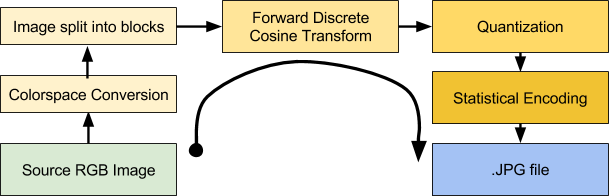
\includegraphics[scale=0.50]{pics/jpegcompression.png}
\caption{Steps involved in JPEG Compression\cite{Jpeg}}
\label{fig:jpeg}
\end{figure}

\begin{figure}[]
\centering
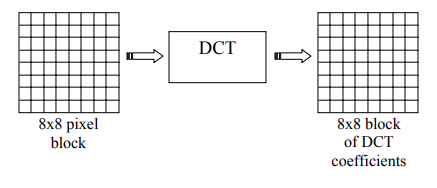
\includegraphics[scale=1]{pics/dct.PNG}
\caption{DCT involved in JPEG\cite{dct}}
\label{fig:dct}
\end{figure}
\subsection{Masks and Reconstruction Algorithms}
The main aim of designing a lensless camera is that it would help reduce the size of the camera considerably. In a lensed camera, light emanating from multiple-points in the object would intersect to form the image of the object. This is illustrated in Figure \ref{fig:lens_image}. The focal length of the lens involved primarily determines the thickness of the camera(See Figure \ref{fig:focal_length}). In a lensless imaging system, the lens is replaced by means of a mask(series of pinholes arranged in a periodic manner). This is illustrated in Figure \ref{fig:lensvslensless}.
\begin{figure}[ht]
\centering
\begin{subfigure}{0.75\textwidth}
  \centering
  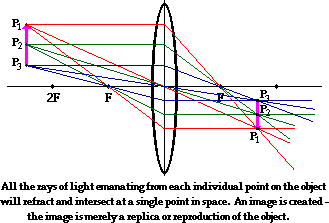
\includegraphics[width=\linewidth]{pics/lensed_image_formation}
  \caption{Image Formation in a lens-based camera\cite{lens1}}
  \label{fig:lens_image}
\end{subfigure}
\begin{subfigure}{1\textwidth}
  \centering
  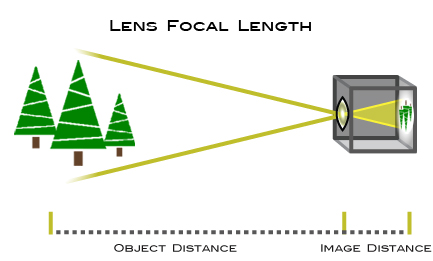
\includegraphics[width=.65\linewidth]{pics/focal_length}
  \caption{Image Distance dictated by focal length \cite{lens2}}
  \label{fig:focal_length}
\end{subfigure}
\caption{Lens-based Camera}
\label{fig:lens_based}
\end{figure}

The simplest lensless imaging system is the pinhole camera. However, since the quality of the image depends on the size of the pinhole, that restricts the amount of light that can enter the imaging system. Lenses were introduced to focus the light from distant objects onto a film or a sensor. In the absence of a lens, the sensor would record the average intensity of the light entering it. This is also seen in the experiments which are described in the upcoming chapters. The difference between pinhole, lensed and a mask-based camera is shown in Figure \ref{fig:flatcam_comp}.
\begin{figure}[ht]
\centering
\begin{subfigure}{\textwidth}
  \centering
  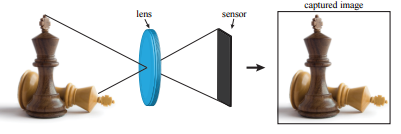
\includegraphics[width=0.75\linewidth]{pics/lensless_1}
  \caption{Conventional Lensed Imaging}
  \label{fig:lensed_imaging}
\end{subfigure}
\begin{subfigure}{\textwidth}
  \centering
  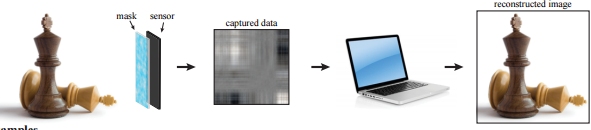
\includegraphics[width=0.75\linewidth]{pics/lensless_2}
  \caption{Lensless Imaging}
  \label{fig:lensless_imaging}
\end{subfigure}
\caption{Difference between lensed and lensless imaging methods\cite{VBoomi}}
\label{fig:lensvslensless}
\end{figure}

\begin{figure}[ht]
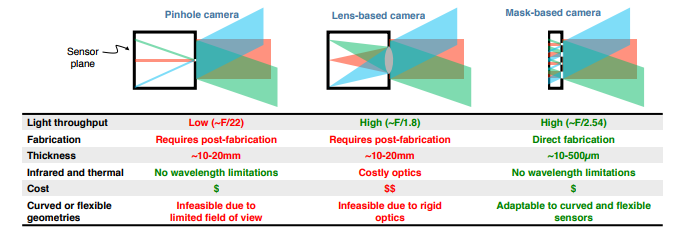
\includegraphics[width=\textwidth]{pics/flatcam_comp}
\caption{Comparison between different types of cameras\cite{Flatcam}}
\label{fig:flatcam_comp}
\end{figure}

In the 1960s, Fernimore and Canon introduced Fresnel Zone Plates for a ``large aperture, high-resolution camera with neither refracting or reflecting components"\cite{Cannon1}. The Fresnel zone plate is defined such that the radius of the $n^{th}$ zone is given by 
\begin{equation}
r_n  = r_1 \sqrt{n}
\end{equation}
An example of Fresnel Zone plate is shown in Figure \ref{fig:fzp}. Fresnel Zone Plates can be used in the places of lenses to produce images because FZPs produce images at multiple higher order foci depending on the type of Fresnel plate used. The Fresnel zone plates have a transmittance(refers to the ratio of light that is entering versus leaving the mask) of exactly 50 percent. It is always desirable to have an optical system with ideal system point spread function(SPSF). The point spread function describes the response of an optical system to a point source. It can also be called as the impulse response of the optical system. The ideal point spread function of an optical system would be a Dirac-delta function. However, in order to obtain such response with a Fresnel zone plate, it would have to be infinite. So, different forms of coded-apertures were developed to overcome the limitations associated with Fresnel zone plates. 

    \begin{figure}[ht]
    \centering
    \begin{subfigure}{0.75\textwidth}
      \centering
      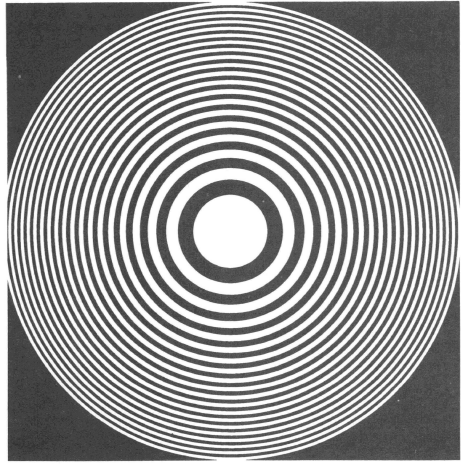
\includegraphics[width=0.350\linewidth]{pics/fzp}
      \caption{A twenty ring Fresnel Zone Plate}
      \label{fig:fzp}
    \end{subfigure}
%\hfill
    \begin{subfigure}{0.75\textwidth}
      \centering
      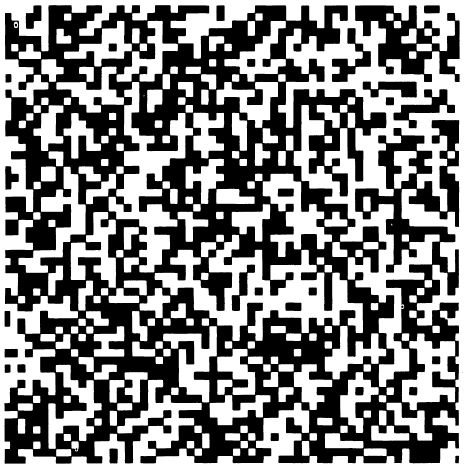
\includegraphics[width=0.350\linewidth]{pics/random_array}
      \caption{A 60*60 Random Array}
      \label{fig:random_array}
    \end{subfigure}
%\hfill
    \begin{subfigure}{0.75\textwidth}
      \centering
      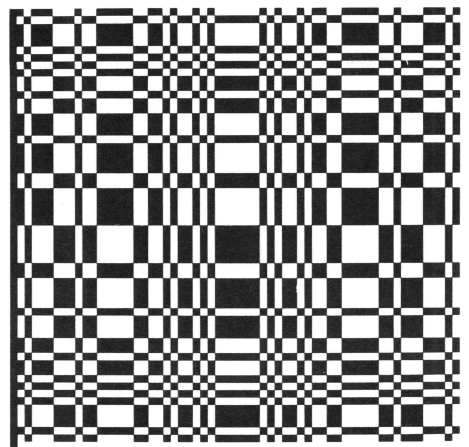
\includegraphics[width=0.350\linewidth]{pics/ura}
      \caption{A 61*59 Uniformly redundant array}
      \label{fig:ura}
    \end{subfigure}

\caption{Masks developed initally for lensless imaging\cite{Cannon1}}
\label{fig:masks_1}
\end{figure}

Coded aperture cameras extend the pinhole camera concept replacing the single aperture with a mask containing multiple apertures. The first developed coded aperture cameras were used in imaging X-Ray sources due to the difficulty involved in focusing light from X-Ray sources\cite{Cannon1}. Since a single pinhole limits the amount of light imaged by the sensing element, it was replaced by many holes, called the aperture so that overlapping images are formed on the film. The recorded image will have no similarity with the source and a digital processing is required to reconstruct the source image or the object. The recorded image is mathematically modeled as a  collection of overlapping shadows as described by the following equation\cite{VBoomi}\cite{Cannon1} 
\begin{equation}
I = M * O + e
\label{eq:conv}
\end{equation}
where $I$ represents the image formed on the sensor, $M$ represents the mask pattern, $O$ represents the irradiance vector or the object and $e$ represents the noise. The $*$ operator represents the convolution operation between the mask an the object. The coded aperture increases the flux that falls on the detector and this leads to an increase in the SNR. The SNR can be as large $\sqrt{N}$, where N represents the number of holes in the aperture\cite{Cannon1}. The increased SNR comes at the cost of computational decoding for the image. We can obtain the actual object image $O$ using the inverse of the mask function. An ideal point spread optical function would produce a Dirac-delta response $M * M^{-1}$.
In 1968, Dicke and Ables\cite{Cannon1} introduced random arrays as an alternative coded aperture imaging method. The mask consists of randomly positioned holes in an opaque surface. An example of a random array is shown in Figure \ref{fig:random_array}. The total open area may or may not be equal to the amount of opaqueness. The image produced by random arrays are decoded digitally using auto-correlation analysis of the encoded images\cite{Cannon1}. Like Fresnel Zone Plates, the random array also exhibits an ideal response when the size of the array is infinite which is practically impossible. A new-class of apertures called uniformly redundant arrays(URAs) was developed over the disadvantages associated with random arrays. The uniformly random arrays exhibit a pattern that follows the equation \ref{eq:ura}\cite{Fenimore:78}. The URA have a dimension of $r$ by $s$ with $r - s = 2$. The equation \ref{eq:ura} takes $I  = mod_ri$ and $J  = mod_rj$($i$ and $j$ represent the array index position in x and y).
\begin{equation}
  M(I,J) =
  \begin{cases}
    0 & \text{if $I = 0$} \\
    1 & \text{if $J = 0$ \& $I\neq 0$} \\
    1 & \text{if $C_r(I)C_s(J) = 1$} \\
    0 & \text{otherwise}\\
  \end{cases}
  \label{eq:ura}
\end{equation}
where $M(I,J)$ represent the values of the mask at co-ordinates $I,J$. A value of 1 indicates that mask is open at that point and a value of 0 indicates that the mask is closed. $C_r$ is given by equation \ref{eq:ura_2}.
\begin{equation}
  C_r(I) =
  \begin{cases}
    1 & \text{if there exists an integer $x$ such that 
    $1<x<r$ 
    such that $I = mod_rx^2$    
    } \\
    -1 & \text{otherwise} \\
  \end{cases}
  \label{eq:ura_2}
\end{equation}

The matrix used for deconvolution(given by equation \ref{eq:decura_2}) is given by the equation \ref{eq:decura}. This kind of array produces an ideal point spread function. The point spread function of different masks discussed above is shown in Figure \ref{fig:psf_old_mask}.
\begin{equation}
  G(I,J) =
  \begin{cases}
    1 & \text{if $M(i,j) = 1$} \\
    -1 & \text{if $M(i,j) = 0$} \\
  \end{cases}
  \label{eq:decura}
\end{equation}

\begin{equation}
O = I * G
\label{eq:decura_2}
\end{equation}

\begin{figure}[ht]
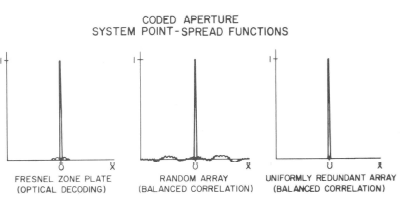
\includegraphics[width=\textwidth]{pics/psf_mask}
\caption{Point Spread function of different masks\cite{Fenimore:78}}
\label{fig:psf_old_mask}
\end{figure}

It can be seen that the Uniformly redundant arrays would offer the best performance and would produce the ideal point spread function. The direct inversion by deconvolution with inverse works when the object is against a dark background with negligible diffraction effects(for example, in the X-Ray Spectrum). 
However, in the later studies\cite{Toeplitz}, it can be seen that equation \ref{eq:conv} no longer holds in the visible light spectrum involving extended-object scenes and direct Fourier/deconvolution based reconstruction methods would fail. This is also observed in the simulation studies described in the upcoming chapter. In order to solve the problems associated with reconstructing extended object scenes in the visible light spectrum, a new class of separable Doubly Toeplitz mask was developed by Michael Et al. \cite{Toeplitz}. These classes of masks retain their properties even in the presence of diffraction and extended-object scene based scenarios. The doubly Toeplitz-masks are expressed as a product of two independent vectors $A$ and $B$.
\begin{equation}
M(i,j) = A(i)B(j)
\end{equation}
If the mask can be expressed in the form of two independent vectors, then the equation \ref{eq:conv} can be re-written in the form: 
\begin{equation}
I = M_AOM_B^T
\label{eq:separable}
\end{equation}

The matrices $M_A$ and $M_B$ are toeplitz meaning they follow the form:

\[ %\arraycolsep=4pt
 M = 
 \begin{bmatrix*}[r]
    A1 & A2 & \cdots &AN & 0 &0 & \cdots & 0 \\
    0 & A1 & A2 & \cdots &AN & 0 & \cdots & 0\\
    \vdots &\cdots &\cdots &\cdots &\cdots&\cdots&\cdots \\
  \end{bmatrix*}
\]

\begin{figure}[ht]
\centering

\includegraphics[scale = 0.50]{pics/doubly-topelitz}
\caption{An example of Doubly-Toeplitz Mask\cite{Toeplitz}}
\label{fig:doubly_toeplitz}
\end{figure}

Previous studies\cite{Toeplitz}\cite{VBoomi}\cite{Flatcam} has proven that it would be possible to perform lensless imaging in the visible light spectrum for real-life object scenes. The detailed solution and modeling of the computational algorithm would be discussed in the next chapter. This kind of mask would be ideal for our application. There is also another class of masks with hexagonal shapes\cite{hexagonal}\cite{hexagonal2} which have been used for coded aperture imaging. However, these have not been studied since they offer no specific advantage compared to other masks discussed above.